%! Author = angel
%! Date = 1/28/25

% Preamble
\documentclass[11pt]{article}

% Packages
\usepackage{amsmath,amssymb,amsthm}
\usepackage{physics}
\usepackage[letterpaper,margin=0.75in]{geometry}
\usepackage{ circuitikz }
\usepackage{pgfplots}
\usepackage{tikz}
\usepackage[dvipsnames]{xcolor}

% Document
\begin{document}
    \noindent \textbf{Chapter 16 - Waves I}
\newline
\newline
    There are three main types of waves:
    \begin{enumerate}
        \item \textbf{Mechanical waves:} governed by Newton's laws, and can only exist
              within physical materials,
              \newline associated with water, sound and seismic waves

        \item \textbf{Electromagnetic waves:} requires no physical medium, and travel at speed $c$  $(3 \times 10^8 m/s)$ in a vacuum,
         associated with light, microwaves, and x-rays
        \item \textbf{Matter waves:} governed by Quantum Physics, particles travel exhibiting both
        wave-like and particle-like behavior, associated with electrons, protons, atoms and matter
    \end{enumerate}

    \noindent Mechanical waves are further classified into how they displace the medium they travel in.
    For example, a speaker playing music displaces air by moving its diaphragm back and forth.
This forward movement pushes air creating an area of compression.
When it moves back, it creates a new area where air is spread out.

\begin{figure}[!ht]
    \centering
    \resizebox{0.5\textwidth}{!}{%
        \begin{circuitikz}
            \tikzstyle{every node}=[font=\LARGE]

            % Wall representation
            \draw [line width=2pt] (18,14) -- (18,10);

            % Velocity purple arrow
            \draw [color={rgb,255:red,255; green,64; blue,255}, line width=1pt, ->, >=Stealth]
            (10.5,13.5) -- (12,13.5);
            \node [font=\LARGE, color={rgb,255:red,255; green,64; blue,255}]
            at (11.3,14) {\textbf{v}};

            % Side-to-side particle movement arrows
            \draw [color={rgb,255:red,4; green,50; blue,255}, line width=1pt, ->, >=Stealth]
            (5.5,12) -- (6.5,12); % Blue left arrow
            \draw [color={rgb,255:red,255; green,38; blue,0}, line width=1pt, ->, >=Stealth]
            (5.5,12) -- (4.5,12); % Red right arrow

            % Compression region (three times as dense in the middle)
            \foreach \x in {5.5, 6, 6.25, 6.5, 6.75, 7,7.1, 7.2, 7.25, 7.3, 7.4, 7.5, 7.6, 7.75, 8, 8.25, 8.5, 8.75, 9, 9.25, 9.5} {
                \draw [short, line width=0.8pt] (\x,12.5) -- (\x,11);
            }

            % Rarefaction region: sparse vertical lines
            \foreach \x in {9.75, 10,10.25, 10.5, 11, 11.5, 12, 12.5, 13, 13.5, 13.75, 14,14.25, 14.5, 14.75} {
                \draw [short, line width=0.8pt] (\x,12.5) -- (\x,11);
            }

            % Compression again near wall
            \foreach \x in {14.9, 15, 15.1, 15.2,15.3,15.35,15.4, 15.5, 15.75, 16, 16.25, 16.5, 17, 17.5} {
                \draw [short, line width=0.8pt] (\x,12.5) -- (\x,11);
            }

        \end{circuitikz}
    }%
    \label{fig:longitudinal_wave}
\end{figure}
\noindent This is known as a \textbf{longitudinal wave} where they displace the medium parallel to the wave’s direction.
Now, imagine a rope with one end in your hand and the other tied to a pole.
   When you move your hand up and down in a harmonic motion,
    the rope forms in the shape of wave as it travels along its length.

\begin{figure}[!ht]
    \centering
    \resizebox{0.4\textwidth}{!}{%
        \begin{circuitikz}
            \tikzstyle{every node}=[font=\LARGE]
            \begin{scope}[rotate around={-1.5:(8.75,11.5)}]
                \draw[domain=8.75:18,samples=100,smooth, line width=1.8pt] plot (\x,{1*sin(1*\x r -8.75 r ) +11.5});
            \end{scope}
            \draw [ line width=1.8pt](18,12.75) to[short] (18,10.25);
            \draw [ color={rgb,255:red,4; green,50; blue,255}, line width=0.8pt, ->, >=Stealth] (8.75,11.5) -- (8.75,12.75);
            \draw [ color={rgb,255:red,255; green,38; blue,0}, line width=0.8pt, ->, >=Stealth] (8.75,11.5) -- (8.75,10.25);
            \node at (8.75,11.5) [circ] {};
            \draw [ color={rgb,255:red,255; green,64; blue,255}, line width=0.8pt, ->, >=Stealth] (10.25,13.25) -- (11.25,13.25);
            \node [font=\LARGE, color={rgb,255:red,255; green,64; blue,255}] at (10.5,13.75) {};
            \node [font=\LARGE, color={rgb,255:red,255; green,64; blue,255}] at (10.75,13.75) {\textbf{v}};
        \end{circuitikz}
    }%

    \label{fig:my_label}
\end{figure}

    \noindent In the case of the rope, the motion is a \textbf{transverse wave}, where the displacement of the medium is perpendicular to the direction the wave travels.

\newpage
    \noindent \textbf{Chapter 16 - Waves I}
    \newline \\ \noindent Both transverse and longitudinal waves are sinusoidal waves where we can find the displacement in the positive $x$ direction modeled by the \textbf{sinusoidal function}:



    \begin{equation}
       \underbrace{y(x,t)}_{\text{\clap{displacement~}}} = \overbrace{y_m}^{\text{\clap{amplitude~}}} sin(\underbrace{kx - \omega t + \phi}_{\text{\clap{phase~}}})
       \tag{displacement} \label{eq:equation}
    \end{equation}



\begin{tikzpicture}
  \begin{axis}[
    trig format plots=rad,
    axis lines = middle,
    enlargelimits,
    clip=false,
    xtick=\empty, % Remove x-axis numbers
    ytick=\empty  % Remove y-axis numbers
    ]
    \addplot[domain=-0.99*pi:2*pi,samples=200,black] {sin(x)};
    \addplot[domain=-2*pi:-1.07*pi,samples=200,black] {sin(x)};
    \draw[dotted,purple,<->] (axis cs: 0.5*pi,1) --  node[above,text=purple,font=\footnotesize]{$y_m$}(axis cs: 0.5*pi,0);
    \draw[dashed,red,<->] (axis cs: 0.5*pi,1.0) -- node[above,text=red,font=\footnotesize]{$\lambda$}(axis cs: -1.5*pi,1.0);

    \draw[dashed,blue,<->] (axis cs: -2*pi,0) -- node[above,text=blue,font=\footnotesize]{$T$}(axis cs: 0,0);
  \end{axis}
\end{tikzpicture}
\hfill
\begin{minipage}[b]{0.5\textwidth}
    Where:
    \begin{itemize}
        \item $y(x,t)$: displacement ($m$)
        \item $y_m$: amplitude ($m$)
        \item $\lambda$: wavelength ($m$)
        \item $f$: frequency ($Hz$)
        \item $T$: period ($s$)
        \item $\omega$: angular frequency ($rad/s$)
        \item $k$: wave number ($m^{-1}$)
        \item $\phi$: phase constant ($rad$)
        \end{itemize}
\end{minipage}
\newline




 \noindent The speed of a wave is dependent on the medium its traveling through as waves travel differently in air than in a rope.
    In fact the velocity of a string under pressure can be calculated by
    finding the \textbf{linear density}
    \begin{equation}
        \mu = \frac{m}{l} \tag{linear density}
    \end{equation}
    Where $m$ is the mass of the string, and $l$ is the length of the string.
    With linear density and the tension force, now we can find the \textbf{velocity.}
    \begin{equation}
        v = \sqrt {\frac{F_T}{\mu}} \tag{wave velocity}
    \end{equation}
    Linear density $\mu$ can also be used to find the \textbf{average power:}
    \begin{equation}
        P_{avg} = \frac{1}{2} \mu v \omega^2 y_m \tag{average power}
    \end{equation}


    \noindent Addition formulas:
    \begin{equation}
        k = \frac{2\pi}{\lambda} \tag{angular wave number}
    \end{equation}
    \begin{equation}
        f = \frac{1}{T} = \frac{\omega}{2\pi} \tag{frequency}
    \end{equation}
    \begin{equation}
        v = \frac{\omega}{k} = \frac{\lambda}{T} = \lambda f \tag{wave velocity}
    \end{equation}
    \begin{align}
        \hspace*{4cm} u = \frac{\partial y}{\partial t} = -\omega y_m\cos(kx-\omega t)\tag{transverse velocity}
    \end{align}
    \begin{equation}
        \frac{\partial^2 y}{\partial x^2} = \frac{1}{v^2} \frac{\partial^2 y}{\partial t^2} \tag{wave equation}
    \end{equation}

    \newpage
    \noindent \textbf{Chapter 16 - Waves I}

    \noindent \\ More than one wave can travel on the same region.
    In fact, when they overlap the waves follow the Principle of Superposition
    where the net displacement is the sum of the displacement from wave one and wave two.
    However, this only affects the displacement, the travel of the wave is untouched.

\begin{minipage}[b]{0.3\textwidth}
    \begin{tikzpicture}
        \begin{axis}[
            ytick=\empty,
            xtick=\empty,
            samples=1000,
            axis line style={draw=none},
            enlargelimits=false,
            height=5cm,
            xmin=-1, xmax=12,
            ymin=-0.05, ymax=4
        ]
            \draw[red,->]
            (axis cs: 1,1.3) -- node[above,text=red,font=\footnotesize]{$$}
            (axis cs: 2.4,1.3);

            \addplot[ line width=0.3mm, color=blue, domain={5:12}, samples=100]
                {(2*pow(2,-1*pow(x-9,2)))};

            \draw[blue,<-]
            (axis cs: 8,2.3) -- node[above,text=red,font=\footnotesize]{$$}
            (axis cs: 9.4,2.3);

            \addplot[ line width=0.3mm, color=red, domain={0:5}, samples=100]
                {(pow(2,-1*pow(x-2,2)))};
        \end{axis}
    \end{tikzpicture}
\end{minipage}
\hfill
\begin{minipage}[b]{0.3\textwidth}
    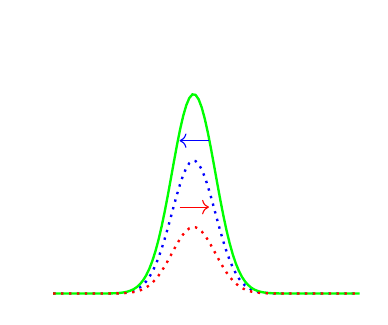
\begin{tikzpicture}
        \begin{axis}[
            ytick=\empty,
            xtick=\empty,
            samples=1000,
            axis line style={draw=none},
            enlargelimits=false,
            height=5cm,
            xmin=-1, xmax=12,
            ymin=-0.05, ymax=4
        ]
            \draw[red,->]
            (axis cs: 4.95,1.3) -- node[above,text=red,font=\footnotesize]{$$}
            (axis cs: 6.1,1.3);

            \addplot[dotted,line width=0.3mm, color=blue, domain={0:12}, samples=100]
                {(2*pow(2,-1*pow(x-5.5,2)))};

            \addplot[line width=0.3mm, color=green, domain={0:12}, samples=100]
            {(3*pow(2,-1*pow(x-5.5,2)))};
            \draw[blue,<-]
            (axis cs: 4.95,2.3) -- node[above,text=red,font=\footnotesize]{$$}
            (axis cs: 6.1,2.3);

            \addplot[dotted, line width=0.3mm, color=red, domain={0:12}, samples=100]
                {(pow(2,-1*pow(x-5.5,2)))};
        \end{axis}
    \end{tikzpicture}
\end{minipage}
\hfill
\begin{minipage}[b]{0.3\textwidth}
    \begin{tikzpicture}
        \begin{axis}[
            ytick=\empty,
            xtick=\empty,
            samples=1000,
            axis line style={draw=none},
            enlargelimits=false,
            height=5cm,
            xmin=-1, xmax=12,
            ymin=-0.05, ymax=4
        ]
            \draw[blue,<-]
            (axis cs: 1,2.3) -- node[above,text=red,font=\footnotesize]{$$}
            (axis cs: 2.4,2.3);

            \addplot[line width=0.3mm, color=red, domain={5:12}, samples=100]
                {(pow(2,-1*pow(x-9,2)))};

            \draw[red,->]
            (axis cs: 8,1.3) -- node[above,text=red,font=\footnotesize]{$$}
            (axis cs: 9.4,1.3);

            \addplot[line width=0.3mm, color=blue, domain={0:5}, samples=100]
                {(2*pow(2,-1*pow(x-2,2)))};
        \end{axis}
    \end{tikzpicture}
\end{minipage}

    \noindent \\ We can calculate the displacement of the \textbf{traveling wave} by adding the displacements of each of the two waves.
    \begin{equation}
        y'(x,t) = y_1(x,t) + y_2(x,t) \tag{displacement of waves}
        \end{equation}

    \noindent Now if two waves are traveling in the same direction where one of them is shifted by $\phi$ radians,
    but have the \textbf{same amplitude and wavelength,} we can calculate the resultant wave:
    \begin{equation}
        y'(x,t) = 2y_{m}\cos(\frac{\phi}{2})\    sin(kx - \omega t + \frac{\phi}{2}) \tag{traveling wave}
    \end{equation}

    \noindent The Principle of Superposition also applies to waves traveling in the opposite direction.
    For a wave traveling in the positive x direction $y_1(x,t) = y_msin(kx - \omega t)$ and another traveling
    in the negative x direction $y_1(x,t) = y_m\sin(kx + \omega t)$, the resultant wave is now a
    \textbf{standing wave}, given by the equation:
    \begin{equation}
        y'(x,t) = 2y_{m}\sin(kx)\cos(\omega t) \tag{standing wave}
    \end{equation}

    \noindent Standing waves bring characteristics that traveling waves do not have.
    These waves have nodes where the two waves intersect, resulting in zero displacement.
    Where the two waves are the farthest apart resulting in the maximum displacement, are known as
    antinodes.
    \newline
     \resizebox{0.3\textwidth}{!}{%
    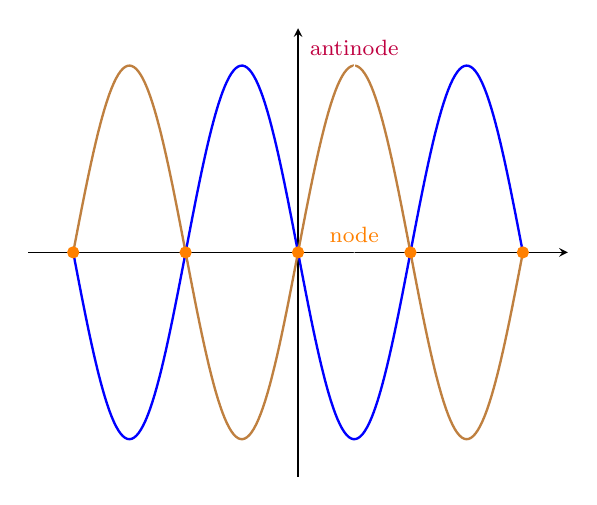
\begin{tikzpicture}
        \begin{axis}[
            trig format plots=rad,
            axis lines = middle,
            enlargelimits,
            clip=false,
            xtick=\empty, % Remove x-axis numbers
            ytick=\empty  % Remove y-axis numbers
        ]
            \addplot[line width=0.3mm, domain=-2*pi:2*pi,samples=200,brown] {sin(x)};
            \addplot[line width=0.3mm,domain=-2*pi:2*pi,samples=200,blue] {sin(x+pi)};
            \draw[dotted,white,->] (axis cs: 0.5*pi,1) --  node[above,text=purple,font=\footnotesize]{antinode}(axis cs: 0.5*pi,1);
            \draw[dotted,white,->] (axis cs: 0.5*pi,0) --  node[above,text=orange,font=\footnotesize]{node}(axis cs: 0.5*pi,0);
            \addplot[only marks, mark=*, color=orange] coordinates {(0,0)};
            \addplot[only marks, mark=*, color=orange] coordinates {(pi,0)};
            \addplot[only marks, mark=*, color=orange] coordinates {(-2*pi,0)};
            \addplot[only marks, mark=*, color=orange] coordinates {(2*pi,0)};
            \addplot[only marks, mark=*, color=orange] coordinates {(-1*pi,0)};
        \end{axis}
    \end{tikzpicture}
    }%
    \hfill
    \begin{minipage}[b]{0.68\textwidth}
       Nodes can be found when $\sin(kx) = 0$ giving the function:
        \begin{equation}
            x = n \frac{\lambda}{2} \tag{node position}
        \end{equation}
        and antinodes can be found using:
        \begin{equation}
            x = (n + \frac{1}{2})\frac{\lambda}{2} \tag{antinode position}
        \end{equation}
        where n is a non-negative integer such as 0,1,2,....
    \end{minipage}

    \noindent \\ Nodes can be used to find \textbf{resonant frequencies}.
    Resonance is when standing waves reaches its maximum amplitude at a specific
    frequency.
    At this frequency, the energy transfer to the medium is at its most efficient.
    \begin{equation}
        f = \frac{v}{\lambda} = n \frac{v}{2L} \tag{Resonant frequency}
    \end{equation}

    \newpage
    \noindent \textbf{Chapter 16 - Waves I}
    \noindent \newline \\ The previous formulas only work if the two waves have the same amplitude.
    If two waves happen to have different amplitudes, we can treat the direction
    of each wave at a given point as a vector.

    \resizebox{0.3\textwidth}{!}{%
        \begin{tikzpicture}
            \begin{axis}[
                ytick=\empty,
                xtick=\empty,
                samples=1000,
                axis lines = left,
                enlargelimits=false,
                height=5cm,
                xmin=-1, xmax=12,
                ymin=-0.05, ymax=4
            ]
                \draw[blue,->]
                (axis cs: -1,0) -- node[above,text=red,font=\footnotesize]{}
                (axis cs: 9.7,2);
                \draw[blue]
                (axis cs: 5,0.3) -- node[above,text=blue,font=\footnotesize]{$y_{m1}$}
                (axis cs: 5,0.3);
                \addplot[dashed,line width=0.3mm, color=red, domain={-6:10}, samples=100]
                {(2*sin(4*pi*x)+0.4)};
            \end{axis}
        \end{tikzpicture}
    }%
    \hfill
    \resizebox{0.3\textwidth}{!}{%
    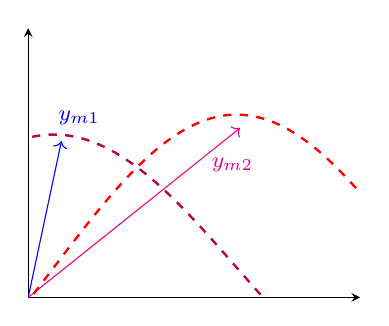
\begin{tikzpicture}
        \begin{axis}[
            ytick=\empty,
            xtick=\empty,
            samples=1000,
            axis lines = left,
            enlargelimits=false,
            height=5cm,
            xmin=-1, xmax=12,
            ymin=-0.05, ymax=4
        ]
            \draw[blue,->]
            (axis cs: -1,-0.05) -- node[above,text=red,font=\footnotesize]{}
            (axis cs: 0.3,2.3);
            \draw[magenta,->]
            (axis cs: -1,-0.05) -- node[above,text=red,font=\footnotesize]{}
            (axis cs: 7.3,2.5);
            \draw[magenta]
            (axis cs: 7,1.7) -- node[above,text=magenta,font=\footnotesize]{$y_{m2}$}
            (axis cs: 7,1.7);
            \draw[blue]
            (axis cs: 1,2.4) -- node[above,text=blue,font=\footnotesize]{$y_{m1}$}
            (axis cs: 1,2.4);
            \addplot[dashed,line width=0.3mm, color=red, domain={-6:12}, samples=100]
            {(2.3*sin(4*pi*x)+0.4)};
            \addplot[dashed,line width=0.3mm, color=purple, domain={-6:12}, samples=100]
            {(2*cos(4*pi*x)+0.4)};
        \end{axis}
    \end{tikzpicture}
    }%
    \hfill
    \resizebox{0.3\textwidth}{!}{%
    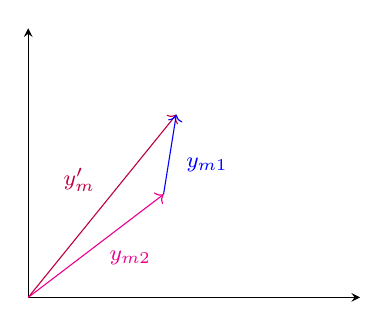
\begin{tikzpicture}
        \begin{axis}[
            ytick=\empty,
            xtick=\empty,
            samples=1000,
            axis lines = left,
            enlargelimits=false,
            height=5cm,
            xmin=-1, xmax=12,
            ymin=-0.05, ymax=4
        ]
            \draw[purple,->]
            (axis cs: -1,-0.05) -- node[above,text=red,font=\footnotesize]{}
            (axis cs: 4.8,2.7);

            \draw[blue,->]
            (axis cs: 4.3,1.5) -- node[above,text=red,font=\footnotesize]{}
            (axis cs: 4.8,2.7);
            \draw[magenta,->]
            (axis cs: -1,-0.05) -- node[above,text=red,font=\footnotesize]{}
            (axis cs: 4.3,1.5);
            \draw[magenta]
            (axis cs: 3,0.3) -- node[above,text=magenta,font=\footnotesize]{$y_{m2}$}
            (axis cs: 3,0.3);
            \draw[blue]
            (axis cs: 6,1.7) -- node[above,text=blue,font=\footnotesize]{$y_{m1}$}
            (axis cs: 6,1.7);
            \draw[purple]
            (axis cs: 1,1.4) -- node[above,text=purple,font=\footnotesize]{$y'_{m}$}
            (axis cs: 1,1.4);
        \end{axis}
    \end{tikzpicture}
    }%
   \noindent \\ \\ \textbf{Phasors} allow us to treat each point as a vector, where we can
    add the two phasors using vector addition.
    Let $y_1 = y_{m1} \sin(kx + \omega t)$ and $y_2 = y_{m2} \sin(kx + \omega t + \phi)$.
    By adding the horizontal and vertical components of each vector we get the resultant vector:
    \begin{equation}
        y'_{m} = \sqrt{y'_{mh} +y'_{mv}} \notag
    \end{equation}
    Where  $y'_{mh}$ is the horizontal component and $y'_{mv}$ is the vertical component
    \begin{equation}
        y'_{mh} = y_{m1}\cos(0) + y_{m2}\cos(\phi) \notag
    \end{equation}
    \begin{equation}
        y'_{mv} = y_{m1}\sin(0) + y_{m2}\sin(\phi) \notag
    \end{equation}

    \noindent In fact we can simplify this equation to:
    \begin{equation}
        y'_{m} = \sqrt{(y_{m1})^2 + (y_{m2})^2 + 2y_{m1}y_{m2}\cos(\phi)} \tag{net amplitude}
    \end{equation}
    
    \noindent The new phase constant is given by:
    \begin{equation}
        \beta = \tan^{-1}({\frac{y_{m2}\sin(\phi)}{y_{m1} + y_{m2} \cos(\phi)}}) \tag{net phase constant}
    \end{equation}

    \noindent Now the net wave function has the form of:
    \begin{equation}
        y'(x,t) =  y'_{m}\sin(kx - \omega t + \beta) \notag
    \end{equation}
\end{document}

